\documentclass{ctexart}
\usepackage{graphicx}
\usepackage{tikz}
\usepackage{caption}
\usepackage{float}
\usepackage{amsmath}
\usepackage{fancyhdr}
\usepackage{xunicode-addon}
\usepackage{booktabs}
\usepackage{listings}
\usepackage{hyperref}
\usepackage{amssymb}
\usepackage[a4paper,hmargin=1.25in,vmargin=1in]{geometry}

% Add the TikZ library "bayesnet"
\usetikzlibrary{bayesnet}

% !TeX program = xelatex
\lstdefinestyle{mystyle}{
  basicstyle=\ttfamily\footnotesize,
  breakatwhitespace=false,         
  breaklines=true,                 
  captionpos=b,                    
  keepspaces=true,                 
  numbers=left,                    
  numbersep=5pt,                  
  showspaces=false,                
  showstringspaces=false,
  showtabs=false,                  
  tabsize=2
}

\lstset{style=mystyle}

\title{\begin{figure}[H]
	\centering 
	\includegraphics[height=7cm,width=14cm]{E:/Pictures/中科大.jpg}
	\end{figure}\Huge\textbf{Homework 3}\\\huge{Bayesian Network}}
\date{}
\punctstyle{banjiao} 
\pagestyle{fancy}
	\fancyhead[C]{\LARGE\textbf{Homework 3}}
	\fancyhead[L]{}
	\fancyhead[R]{}
	\fancyfoot[C]{\thepage}
\begin{document}
	\maketitle
	\thispagestyle{empty}
	
	\[\makebox{\Large{姓名:\underline{\makebox[5cm]{高茂航}}}}\]
	
    \[\makebox{\Large{学号:\underline{\makebox[5cm]{PB22061161}}}}\]
	
	$$\makebox{\Large{日期:\underline{\makebox[5cm]{2024.6.1}}}}$$
	
	\clearpage

	\pagenumbering{arabic}

	\section{概率推断[25\%]}
	\subsection{}
	\begin{figure}[h]
		\centering
		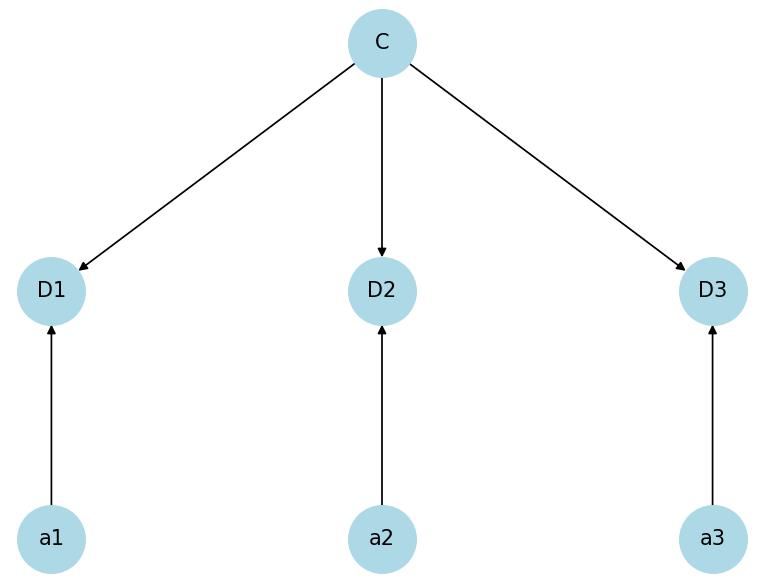
\includegraphics[height=6cm,width=10cm]{1.png}
		\end{figure}
		\subsection{}
		$\because D_t$ 只依赖于C和$a_t$,

		$\therefore P(C = c, D_1 = d_1, D_2 = d_2, D_3 = d_3) = P(C = c)P(D_1 = d_1 | C = c, a_1) P(D_2 = d_2 | C = c, a_2) P(D_3 = d_3 | C = c, a_3)$
		\subsection{}
		\begin{align*}
			P(C = c|D_1 = d_1, ..., D_t = d_t) &= \frac{P(C = c, D_1 = d_1, ..., D_{t-1}= d_{t-1}, D_t = d_t)}{P(D_1 = d_1, ..., D_{t-1} = d_{t-1}, D_t = d_t)}\\
			&= \frac{P(C = c)P(D_1 = d_1|C=c)P(D_2 = d_2|C=c) ...P(D_t = d_t|C=c)}{P(D_1 = d1, ..., D_{t-1} = d_{t-1}, D_t = d_t)}\\
			&= \frac{P(C = c,D_1 = d_1, . . . , D_{t-1} = d_{t-1})P(D=d_t|C = c)}{P(D_1 = d_1, ..., D_{t-1} = d_{t-1}, D_t = d_t)}\\
			&= \frac{P(C = c|D_1 = d_1, ..., D_{t-1} = d_{t-1})P(D=d_t|C = c)}{P(D_t=d_t|D_1 = d_1, . . . , D_{t-1} = d_{t-1})}\\
			& \propto P(C = c|D_1 = d_1, ..., D_{t-1} = d_{t-1})P(D=d_t|C = c)
		\end{align*}

		\section{转移概率[25\%]}
		\subsection{}
		\begin{figure}[H]
			\centering
			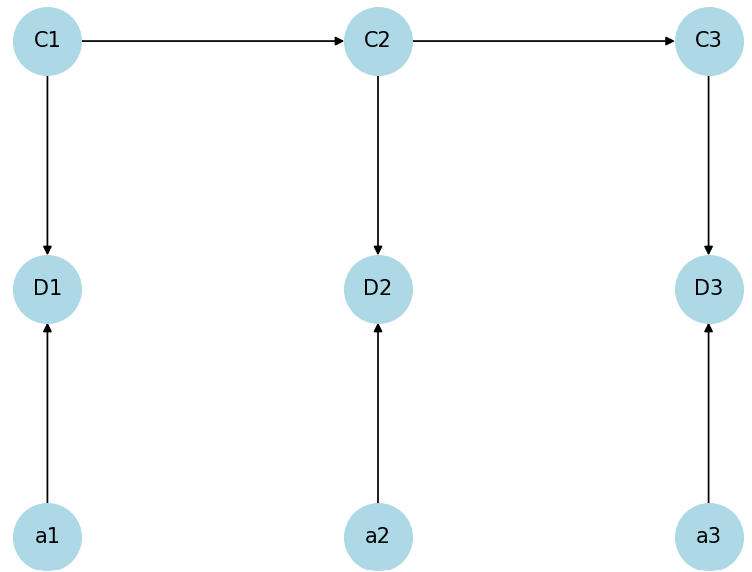
\includegraphics[height=6cm,width=10cm]{2.png}
			\end{figure}
			\subsection{}
			$\because D_t$ 依赖于$C_t$和$a_t$,且$C_t$依赖于$C_{t-1}$,
			
			$\therefore P(C_1 = c_1, C_2 = c_2, C_3 = c_3, D_1 = d_1, D_2 = d_2, D_3 = d_3) =P(C_1 = c_1) P(D_1 =d_1 | C_1 = c_1) P(C_2 = c_2 | C_1 = c_1) P(D_2 = d_2 | C_2 = c_2) P(C_3 = c_3| C_2 = c_2) P(D_3 =d_3| C_3 = c_3)$
			\subsection{}
			\begin{align*}
				P(C_{t+1} = c_{t+1}|D_1 = d_1, ..., D_t = d_t) 
				&= \frac{P(C_{t+1} = c_{t+1}, D_1 = d_1, ..., D_{t-1}= d_{t-1}, D_t = d_t)}{P(D_1 = d_1, ..., D_{t-1} = d_{t-1}, D_t = d_t)}\\
				&= \sum\limits_{c_t}\frac{P(C_{t+1} = c_{t+1}, C_t = c_t, D_1 = d_1, ..., D_{t-1}= d_{t-1}, D_t = d_t)}{P(D_1 = d_1, ..., D_{t-1} = d_{t-1}, D_t = d_t)}\\
				&= \sum\limits_{c_t}\frac{P(C_t = c_t,D_1 = d_1, . . . , D_t = d_t)P(C_{t+1}=c_{t+1}|C_t = c_t, ..., D_t = d_t)}{P(D_1 = d_1, ..., D_{t-1} = d_{t-1}, D_t = d_t)}\\
				&= \sum\limits_{c_t}\frac{P(C_t = c_t,D_1 = d_1, . . . , D_t = d_t)P(C_{t+1}=c_{t+1}|C_t = c_t)}{P(D_1 = d_1, ..., D_{t-1} = d_{t-1}, D_t = d_t)}\\
				& \propto\sum\limits_{c_t} P (C_t = c_t|D_1 = d_1, …, D_t = d_t)P(C_{t+1}=c_{t+1}|C_t=c_t)
			\end{align*}
	
			

	\section{是哪辆车?[30\%]}
	\subsection{}
	\subsection{}
	\subsection{}
	\subsection{}
	\section{模型学习[10\%]}
	\subsection{}
	\section{反馈[10\%]}
	
	



	

\end{document}